\section{Test vehicule description and failure signature}

This chapter focuses on the functionnal failure caused by an \gls{esd} of an integrated function.
The studied function is the primary supply of a complex automotive \gls{asic}.
This supply plays a critical role in the functionning of the entire product.
It is connected to the battery of the vehicle, and is the first block of the product to start.
It wakes up and powers all other functions inside the integrated circuit.

\begin{figure}[h]
  \centering
  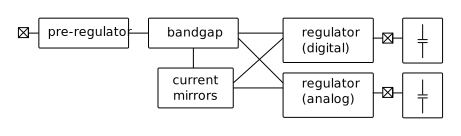
\includegraphics{src/4/figures/testchip_overview.pdf}
  \caption{Architecture of the studied functionnality}
  \label{testchip_overview}
\end{figure}

The primary supply processes the battery supply in a chained fashion (see Fig. \ref{testchip_overview}).
A first block (pre-regulator) clamps the battery voltage (that can reach up to 40V) to 9V, a more acceptable voltage for the silicium technology.
This clamped voltaged is then used to power up a bandgap reference.
Once properly started, this bandgap generates a 1.23 V voltage reference, stable accross a wide range of temperature, process variation and mismatchs.
The bandgap also outputs a 10uA current reference, stable in the same conditions.

After the bandgap, a \gls{ldo} regulator relies on the voltage reference to generate a stable 2.5V supply voltage, able to deliver and sustain up to 20mA.
This first regulator is connected externally to a 100nF decoupling capacitor to absorb peak currents and achieve stability.
This supply is used to supply most analog (digital ?) functions inside the integrated circuit.

A second regulator performs the same task, but starts with a delay compared to the first one.
It also ouputs a 2.5V supply, that powers digital logic inside the circuit.

In case of failure, the primary supply can cause the entire product to shut down.
Indeed, this entire system requires soft-start behavior to avoid generating harmful voltage spikes to powered functions.
This functionnality enforces the system to start on a \br{long} period of time, in the order of a hundred microseconds.

When the system is stressed with an \gls{esd}, voltages and currents are fluctuating inside the block.
Under certain conditions, and especially important stress levels, the block will detects some nodes going in undervoltage or overvoltage.
This will cause the block to go into safe or protected mode, where it will restart because the functionnality cannot be assured properly.
The direct consequence is that the block will require again a hundred microseconds to be again in normal operation mode.

This failure can in a first time be observed in simulation.
An \gls{ESD} is superimposed on the DC battery voltage.
This is the most likely entry point for a stress, because the \gls{IC} exposes a pin to the external workd and is usally connected to the battery via a long cable
To detect is a block reset happened, the voltage on the first voltage regulator is observed.
Fig. X shows the stress waveform on the input.

STRESS WAVEFORM INPUT

Fig. X shows a simulation where a small glitch can be observed on the regulated output, but without clear reset or soft-failure signature.
In this case, the block and the rest of the product is most likely not affected by the ESD.

WAVEFORM OUTPUT NO RESET

Fig. X shows a simulation where a clear reset hapened.
The output voltage is maintained by a 100nF capacitor.
However, it clearly goes down \br{after} the \gls{esd} and rises slowly afterward, a sign that the block went into full reset and restard.

WAVEFORM OUTPUT RESET

By going inside the \gls{IC}...

bandgap, voltage ref, current ref, etc

DISCUSSION AROUND INCREASE OF FAILURE LENGTH after each stage of the chain

\section{Bottom-up block failure modeling}

Consider a system constituted of two blocks A and B connected together.

\begin{figure}[!htbp]
  \centering
  
\includegraphics{src/4/figures/system_ab.pdf}
  \caption{Basic IC function}
  \label{basic_ic_function}
\end{figure}

During normal operation, the \textbf{\textit{out}} signal complies with its specification,
under the condition that the \textbf{\textit{in}} signal does too.
This guarantees that block A and B are performing as expected.

When the system is exposed to an electrical stress on the input during normal operation,
the \textbf{\textit{in}} signal is disturbed.

It no longer complies with its specification, for a given amount of time.

The robustness of the entire system is defined by its ability to maintain signal \textbf{\textit{out}} in specification
while signal \textbf{\textit{in}} is temporarily disturbed.

Time is a key parameter here. On one extreme side, a disturbance that lasts forever is equivalent to the \textbf{\textit{in}} signal not fullfilling its DC specification,
and thus the \textbf{\textit{out}} signal will not fullfill its spec as well.
On the other extreme side, an extremely short disturbance, much shorter than the functionnal timescales of the integrated function will most likely not disturb ??

The first task for defining the robustness of an integrated function is to determine the time threshold under which it can maintain functionnality while being disturbed.
The second key parameter is related to the amplitude of the disturbance, whether it is a voltage, current, energy, etc.
A larger amplitude can make a short pulse more harmful than a lomg one.

\subsection{Block characterization method}

In a bottom-up approach, the study starts on the small-scale components,
later assembled together to reach higher levels of complexity.

This method fits well with the integrated circuit design flow in general,
where blocks are build from transistors and other devices, then assembled together to build interesting functionnalities.

The main perk of this characterization method is its modularity.
Each block can be studied independently.
It complies well with a block-reuse design flow as well.
A characterized block can be reused multiple times without having to re-do the characterization.

Blocks are characterized in a particular setup, and their own robustness is deduced. The final goal is to determine if the robustness of
a system can be assimilated as the sum of the robustness of its parts.

The studied block is placed under normal operating conditions. EXPLAIN MORE.

An input and output pin of interest are selected according to the block's connection inside the chain constituting the total function.
Fix. \ref{block_function_cz} gives an example of such a characterization setup.

\begin{figure}[!htbp]
  \centering
  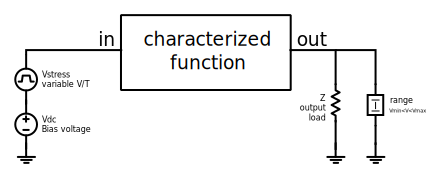
\includegraphics{src/4/figures/characterization_setup.pdf}
  \caption{Block function characterization setup}
  \label{block_function_cz}
\end{figure}

The block is then stressed with a square impulse of variable length and variable amplitude.
Such stress method is called Wunsch & Bell in the litterature (REFERENCE).

The goal is to find out, for each stress duration, what is the minimal voltage \textbf{\textit{V(in)}} required to make the block fail.

Fix. \ref{wb_cz_curve_example} gives an example of such a characterization curve.

\begin{figure}[!htbp]
  \centering
  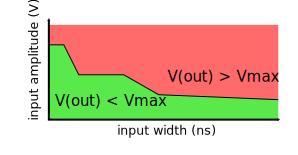
\includegraphics{src/4/figures/example_curve.pdf}
  \caption{Principle of Wunsch & Bell curve for powered-on block testing}
  \label{wb_cz_curve_example}
\end{figure}

The main limitation of this curve is the lack of information on how long the output was disturbed.

If the output is only disturbed for a picosecond, then the failure is most certainly less severe than if it was for a millisecond.

To account for this information, a gradient can be used rather than a simple above/below Vmax curve.
For each point of the curve, the gradient will have a value reprensting the duration of the failure on \textbf{\textit{V(out)}}.
The figure \ref{wb_cz_curve_example_v2} warmer the gradient, the longer the output was disturbed.

\begin{figure}[!htbp]
  \centering
  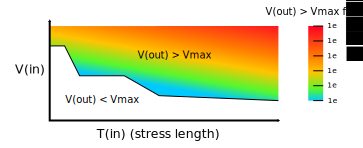
\includegraphics{src/4/figures/example_curve_v2.pdf}
  \caption{Improved curve for Wunsch & Bell powered-on characterization}
  \label{wb_cz_curve_example_v2}
\end{figure}

The gradient can also be discretized into a few aeras for better readability as shown in figure \ref{wb_cz_curve_example_v2_discrete}.
This representation looses some information compared to the gradient one, but is easier to generate and read.
This is the representation we have adopted in the next section, to express the functionnal robustness of a block.

\begin{figure}[!htbp]
  \centering
  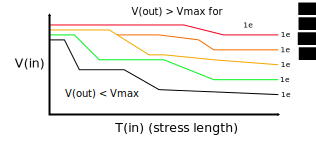
\includegraphics{src/4/figures/example_curve_v2_discrete.pdf}
  \caption{Improved discrete curve for Wunsch & Bell powered-on characterization}
  \label{wb_cz_curve_example_v2_discrete}
\end{figure}

\subsection{Models assembly for full-function robustness}

The method described in section 4.2.1 is is performed in simulation on the regulation function of the testchip.

This function is composed mainly of three blocks, a pre-regulator, a bandgap and a regulator.

In a first time, a very naive approach is used for the characterization load Z (see figure \ref{block_function_cz}) placed on the output of each block.
An arbitrary load value of 1MΩ is chosen. WHY ?

Like explained previously with Vmax (TO CALL Verr ?) in 4.2.1, a failure treshold is chosen for each block.
Under this threshold, the output of each concerned block is considered at fault.

DETAIL MORE SIMULATION PROCESS. PARAMETERIZED SIMULATION WITH MULTIPLE AMPLITUDE/LENGTH

The characterization curves are given in figs. \ref{pre_regu_wb}, \ref{bandgap_wb} and Z.
For the given testchip, it was found that the regulation function shows clear failure when exposed to negative stresses.
For simplicity, the voltage scale was simply reversed, but this doesn't affect the results in any case.

TODO: REVERT Y SCALE ON ALL CURVES

\begin{figure}[!htbp]
  \centering
  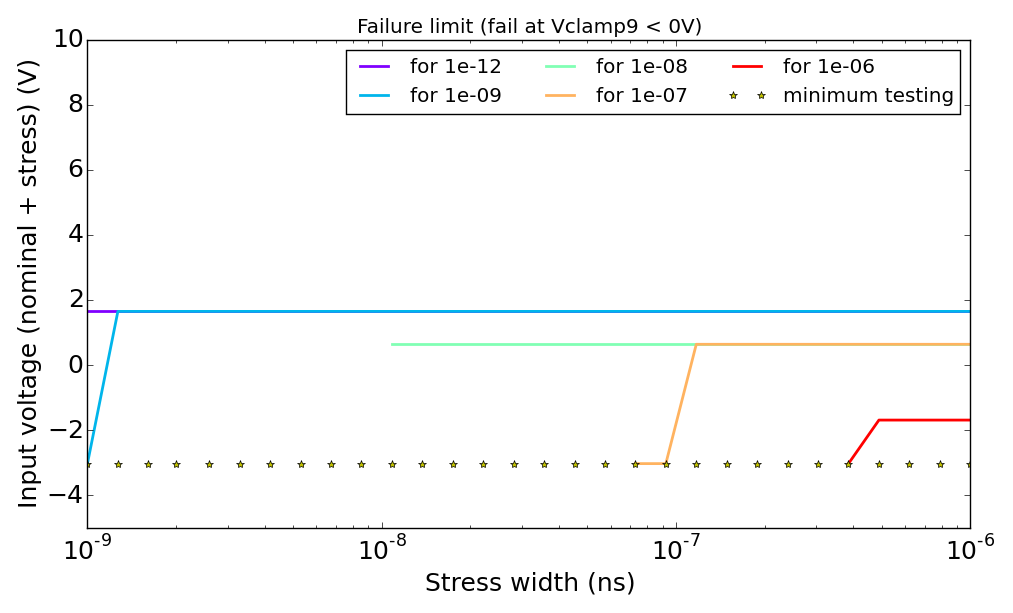
\includegraphics[width=\textwidth]{src/4/figures/cz_vpre.png}
  \caption{Testchip's pre-regulator Wunsch & Bell characterization}
  \label{pre_regu_wb}
\end{figure}

\begin{figure}[!htbp]
  \centering
  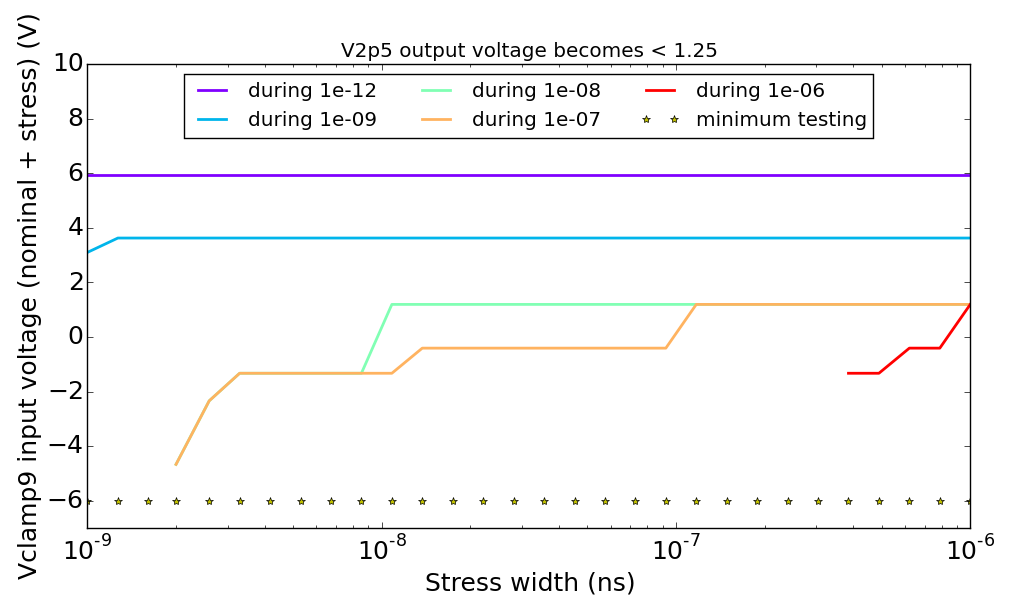
\includegraphics[width=\textwidth]{src/4/figures/cz_bandgap.png}
  \caption{Testchip's bandgap Wunsch & Bell characterization}
  \label{bandgap_wb}
\end{figure}


CURVE CZ REGULATOR

The goal now is to link those curves together, in order to predict if an input
stress applied on the first block can affect the final functionnality outputed
on the last block.

This technique can be done manually in a first time. To validate it,
a simulation is run on the entire schematic will all three blocks
connected together (see Fig. X).
An ESD is injected on pin X, and the functionnality on pin Y is monitored for resets.
The result of this simulation and especially the minimal stress amplitude serves as reference.

SCHEMATIC FULL CIRCUIT

On the other side, the curve method is used to try to reach the same level.
The ESD stress is generated by a TLP of 100ns pulse length and XX V pulse amplitude.
This corresponds on the pre-regulator characterization curve to a point of coordinates (100 ns, XX V).
On the curve, the position of this point shows that in this situation the first block will be at fault (output < X V) for 300? ns.

This gives the coordinates for a point on the second curve (bandgap).
Indeed the output of the first block (regulator) is connected to the input of the second block (bandgap).
This means that we can use directly the point (300ns?, X V) on the second curve to find out if the bandgap will be disturbed.
On the second curve, the position of this point means the bandgap will be at fault (below 0V) for 500ns ?

Repeting this technique on the third curve, we can determine with the characterization that the regulator will be at
fault (below XX V) during XXXX ns.

It is very noticeable that after the second block, the model predicted a failure at
XXX volts while in the complete simulation it is much smaller than that.
Already with a rather simple case, it seems that this method will have some important issues to overcome.

The main issue with this modelling method is the fact that it relies too much
on the value of the output load for performing the characterization of a block.
This load depends on many different parameters.
And this value will change in function out the block connected on the output (think about block-reuse)
Also, this value may not be constant in frequency and in time (during the ESD impulse).

Another issue, this method is limited to a binary FAIL/NO FAIL criteria.
Not only this criteria is arbitrary (in some cases, the specification could be used to set it), but
for most purely-analog blocks, there will not be a clear failure, rather, most
nets will have degraded values until maybe biasing of the block completely fails.
In this case, the binary criteria hides a lot of information about the degradation.

ANY CLUES TO OVERCOME THESE ISSUES ?

The main reason why this approach was investigated was for its very interesting modularity
that was highly suitable for block reuse workflow.

However, because of the intrisic interactions between block functions in an integrated circuit,
this approach seems to be bound to fail for building a reusable model for an IC block that could predict
ESD failures at the architecture level and during the IC architecture phase.
